\documentclass[12pt, a4paper,twoside]{article}
% \usepackage{nicefrac}
% \usepackage[lmargin=3cm,rmargin=2.1cm,tmargin=2.4cm,bmargin=2.4cm]{geometry}
\begin{document}
\label{sec:Tentative Plan}
	As we have achieved good performance for the sensor detection problem, now the part which is left in the matching layer is to train a network to which is able to match images when they are from  different images.
	and since the alignment part has been done now I will be focusing more on how to increase the performance of the alignment network. Finally after the completion of these two phases my main motive would be to find a suitable solution for indexing phase (how to arrange the clusters containing similar binary vectors) and finally training the network which can generate binary vectors. After the completion of these four phases I will try to make a single network pipeline which is backpropagable which can increase the performance of our network.

\begin{figure}[htbp]
\centering
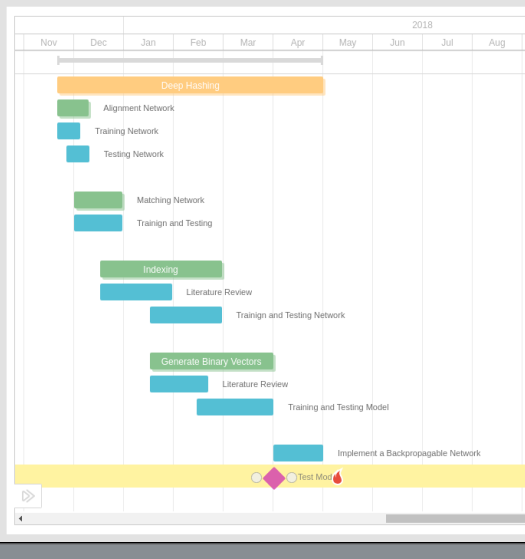
\includegraphics[scale=1]{images/GantChart}
\caption{ Tentative Schedule.
}\label{fig:figure9}
\end{figure} 


\end{document}